\section{Mininet y Mininet-WiFi}
\label{sec:mininet}

En esta sección se abordará el marco teórico relacionado con las principales herramientas de emulación utilizadas en este proyecto. Se prestará especial atención a Mininet, que es la herramienta principal y la base sobre la cual han surgido otras herramientas de emulación, como Mininet-WiFi y Mininet-IoT.\\

\subsection{Mininet}

Mininet es una herramienta utilizada para emular redes, principalmente del tipo SDN (Software-Defined Networking). Permite emular hosts, routers, switches y enlaces en una sola máquina a un coste reducido, siempre y cuando se cuente con el Kernel de Linux en dicha máquina. Para lograr esto, Mininet utiliza una forma de virtualización "ligera" que aprovecha las capacidades del Kernel de Linux para virtualizar recursos, como las \textit{Namespaces} (consultar \ref{namespaces}) \cite{lantz2010network}.\\
\\
La cantidad de recursos virtualizados dependerá de las características de cada nodo, y esto también afectará el rendimiento de la emulación. Por ejemplo, los nodos tipo \texttt{Host} en Mininet requieren el uso de una \textit{Network Namespace}, lo que les proporciona su propio \textit{stack} de red y los hace completamente independientes\footnote{En lo que respecta a Networking} del sistema y otros nodos en la red emulada. Sin embargo, por defecto, todos los nodos \texttt{Host} comparten el sistema de archivos, la numeración de procesos (PIDs), los usuarios, etc. En términos técnicos, no están completamente aislados como un host real. Esto se debe a que Mininet virtualiza solo los recursos necesarios para llevar a cabo la emulación, lo que mejora el rendimiento y permite que máquinas con recursos limitados puedan realizar la emulación \cite{lantz2010network}.\\
\\
En cuanto a la creación de topologías en Mininet, existen dos enfoques. El primero es utilizar la API escrita en Python para interactuar con las clases de Mininet. Con esta API, se puede construir la topología importando los módulos y clases necesarios para definirla en un script de Python. El segundo enfoque es utilizar la herramienta llamada \textbf{MiniEdit}, que proporciona una interfaz gráfica (GUI) donde los usuarios pueden crear la topología arrastrando y soltando nodos de red. Desde la misma GUI, se puede exportar la topología generada a un archivo (\texttt{*.mn}) para recuperarla más tarde o a un script en Python (\texttt{*.py}) para cargarla en el intérprete de Python cuando sea necesario. Esta herramienta es especialmente útil para aquellos que no tienen conocimientos de programación en Python pero desean utilizar el emulador, lo que representa una ventaja significativa \cite{lantz2010network}.\\

Por lo tanto, se puede concluir que los aspectos más fuertes de Mininet son los siguientes puntos:

\begin{itemize}
    \item Mininet es rápido gracias a su diseño basado en \textit{Namespaces}, lo que permite una gestión eficiente de los recursos. En la sección \ref{namespaces}, se explica cómo se lleva a cabo esta gestión.
    \item Mininet no consume recursos en exceso, ya que virtualiza únicamente los componentes necesarios para la emulación. Además, se pueden establecer límites máximos de recursos para la emulación en caso de ser necesario.
    \item Mininet brinda libertad al usuario para crear topologías y escenarios personalizados utilizando la API en Python de Mininet. Estos escenarios pueden ser fácilmente transferidos a otra máquina, ya que solo se requiere compartir el script que describe la topología. Es importante tener en cuenta que los resultados de las pruebas pueden variar entre diferentes máquinas, ya que Mininet emula la red en lugar de simularla. Por lo tanto, los resultados dependerán de las condiciones de la máquina donde se ejecuten las pruebas.
\end{itemize}

Aunque Mininet ofrece muchas ventajas, también tiene una limitación importante que debe tenerse en cuenta. Como se mencionó anteriormente, Mininet utiliza una forma de virtualización ``ligera" basada en las \textit{Namespaces} del Kernel de Linux. Si bien esta decisión de diseño proporciona beneficios significativos en términos de rendimiento al aprovechar el propio sistema operativo para virtualizar recursos, surge un problema cuando se intenta exportar el emulador a otra plataforma con un sistema operativo diferente. Es posible que este sistema operativo no admita un equivalente funcional a las \textit{Namespaces} de Linux o, incluso si lo hace, su API para utilizarlas puede ser completamente diferente. Esto puede dificultar o incluso impedir la ejecución de Mininet en plataformas que no porten el kernel de Linux.


\subsection{Funcionamiento de Mininet}

Anteriormente se mencionó que Mininet utiliza \textit{Network Namespaces} como método para virtualizar \textit{stacks} de red independientes y así emular redes con un costo mínimo. En la figura \ref{fig:mininet_arch}, se muestra la arquitectura interna de Mininet para una topología compuesta por dos nodos \texttt{Host} y un software switch conectado por TCP a un controlador remoto.\\
\\
Como se puede observar, cada nodo \texttt{Host} está aislado en su propia \textit{Namespace} de red, mientras que el switch se ejecuta en la \textit{Namespace} por defecto (root). La comunicación entre los nodos de esta topología se realiza mediante \gls{veth}s (consultar \ref{linuxVeths}), las cuales permiten emular los enlaces entre los diferentes nodos de la red.\\

%fig
\begin{figure}[ht]
    \centering
    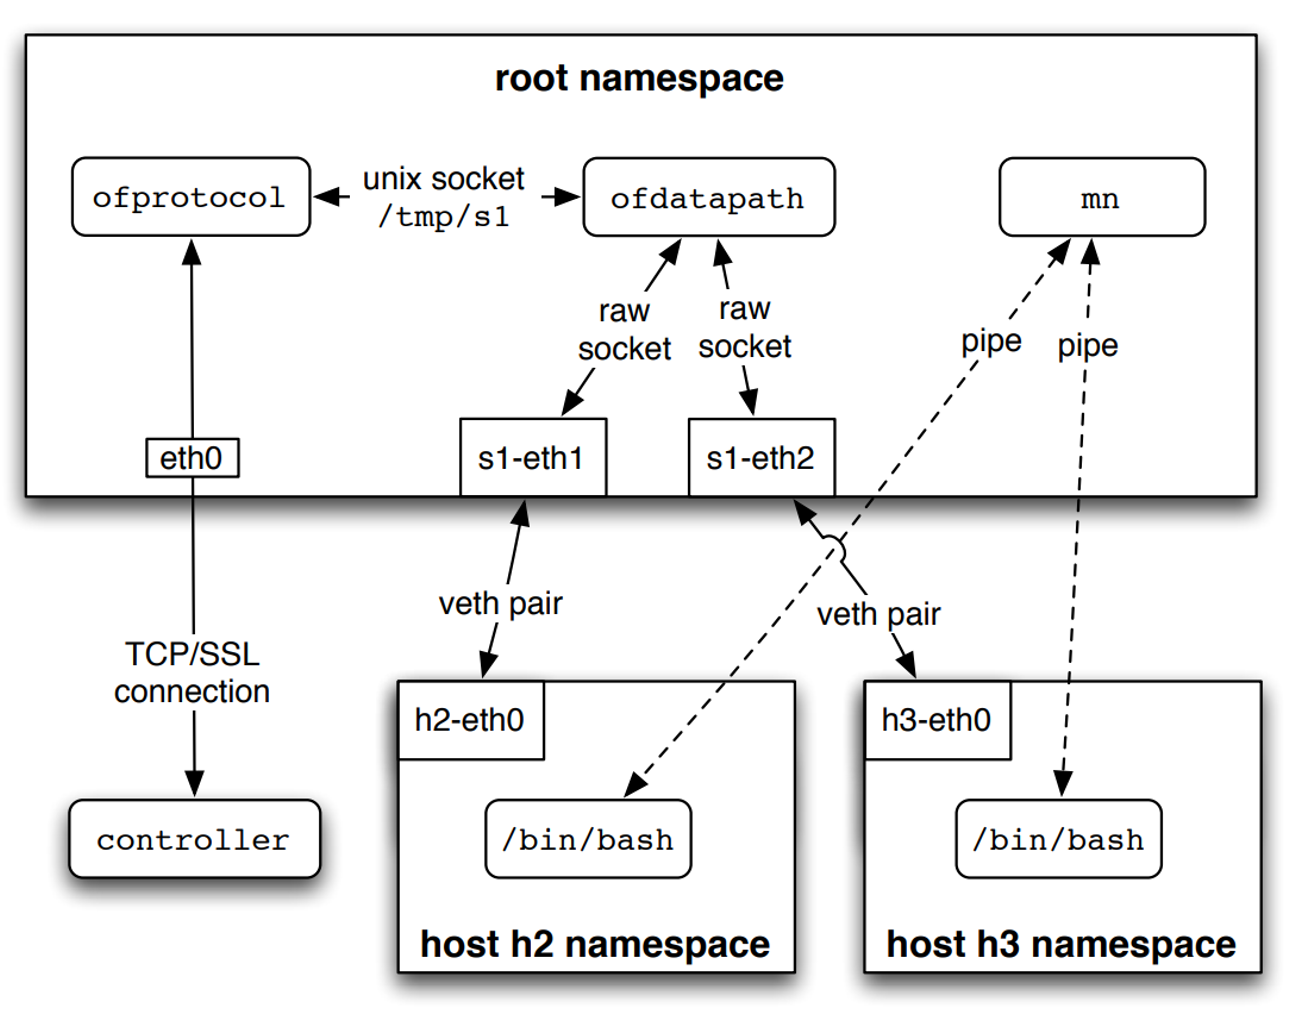
\includegraphics[width=\textwidth]{archivos/img/teoria/mn_arch.png}
    \caption{Arquitectura de Mininet \cite{heller2013reproducible}}
    \label{fig:mininet_arch}
\end{figure}

Una vez presentada toda la teoría sobre Mininet, puede surgir la pregunta de cómo se puede comprobar si realmente utiliza \textit{Network Namespaces}. Para hacerlo, lo primero que se debe hacer es crear el escenario para que Mininet pueda crear las \textit{Network Namespaces} necesarias. En este caso, se utilizará la topología mostrada en la figura \ref{fig:mininet_arch}. Para crear esta topología, solo se necesita tener Mininet instalado y seguir los pasos que se indican en el bloque \ref{code:scenarioMininet}. Una vez levantado el escenario, se debería obtener el output indicado en la figura \ref{fig:mininet_01}.


\begin{lstlisting}[language= bash, style=Consola, caption={Ejecución de Mininet con la topología por defecto},label=code:scenarioMininet]
    # Lanzamos Mininet con la topo por defecto :)
    sudo mn
    
\end{lstlisting}
\vspace{0.5cm}

\begin{figure}[ht]
    \centering
    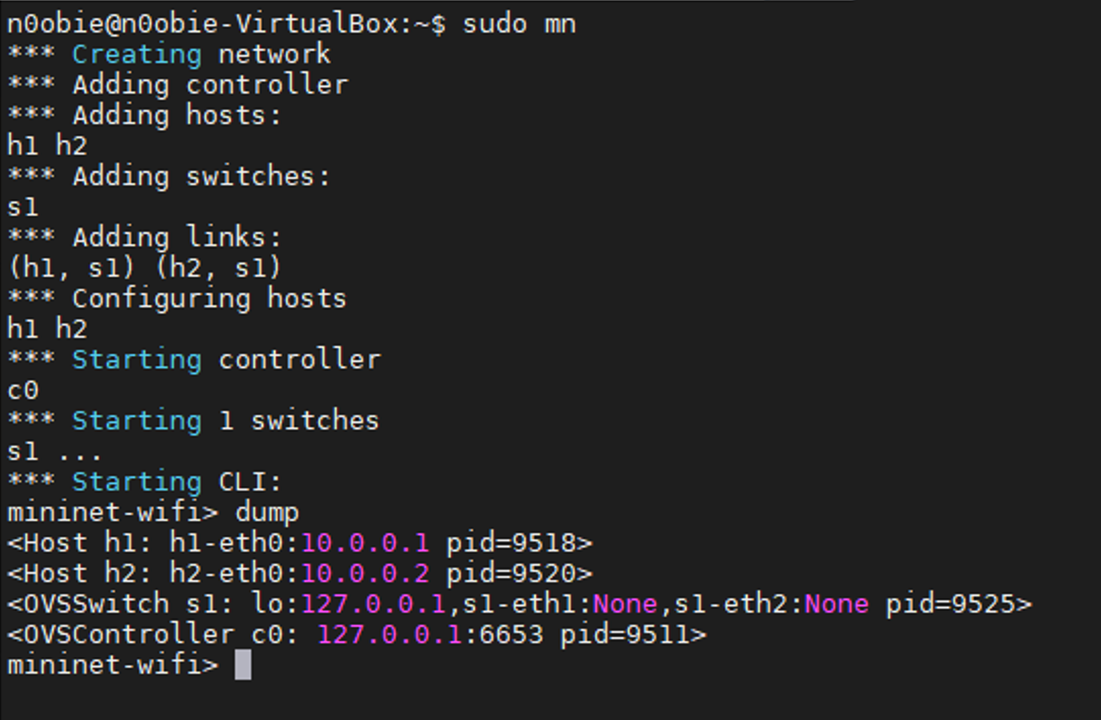
\includegraphics[width=0.7\textwidth]{archivos/img/teoria/mn_01.png}
    \caption{Salida por pantalla de la ejecución de la topología por defecto}
    \label{fig:mininet_01}
\end{figure}

Ahora que hemos creado el escenario, podemos verificar si hay \textit{Network Namespaces} en el sistema utilizando el conjunto de herramientas iproute2 (consultar \ref{iproute2}). El comando más utilizado para listar las \textit{Network Namespaces} utilizando el módulo \textbf{netns} se muestra en el bloque \ref{code:MininetNs}.


\begin{lstlisting}[language= bash, style=Consola, caption={Listar Named Network Namespaces},label=code:MininetNs]
    # Listamos las network namespaces con Nombre! ojito :)
    sudo ip netns list
\end{lstlisting}
\vspace{0.5cm}

\begin{figure}[ht]
    \centering
    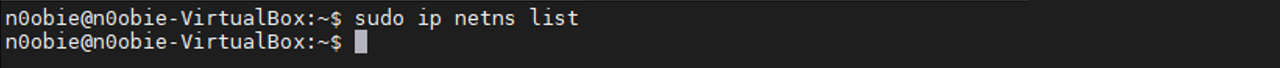
\includegraphics[width=\textwidth]{archivos/img/teoria/mn_02.png}
    \caption{Listado de Named Network Namespaces existentes en el sistema}
    \label{fig:mininet_02}
\end{figure}


Al observar la figura \ref{fig:mininet_02}, no parece haber ninguna \textit{Network Namespace} en el sistema. Entonces, ¿dónde está el problema? La razón por la que el comando \texttt{ip netns list} no muestra información es que Mininet no está creando el enlace simbólico (\textit{softlink}) necesario para que la herramienta pueda listar las \textit{Network Namespaces}. Según la documentación del comando, este lee desde la ruta \texttt{/var/run/netns/}, donde se encuentran todas las \textit{Network Namespaces} con nombre. Estas Netns son aquellas en las que se ha realizado un \textit{bindmount} con su nombre en ese directorio para que persistan incluso si no hay ningún proceso en ejecución en ellas.Como se mencionó anteriormente, las \textit{Namespaces} tienen una vida finita y solo existen mientras estén referenciadas (consulte la tabla \ref{tab:linux_ns}). Por lo tanto, si no se cumple ninguna condición de referencia, la \textit{Namespace} en cuestión se elimina.\\
\\
Mininet se encarga de recrear la red emulada y, cuando el usuario finaliza la emulación, la red emulada debe desaparecer. Este proceso debe ser lo más rápido y eficiente posible para brindar una mejor experiencia al usuario. La naturaleza del diseño de Mininet sugiere que la creación y destrucción de las \textit{Network Namespaces} están asociadas con la primera condición de referencia de una \textit{Namespace}.\\
\\
En otras palabras, no tendría sentido realizar enlaces o enlaces simbólicos que luego se deban eliminar, ya que esto implicaría una carga de trabajo significativa para emulaciones de redes grandes y aumentaría el tiempo necesario para limpiar el sistema una vez finalizada la emulación. Además, hay que tener en cuenta que existe una condición que se adapta bien a las necesidades de Mininet: solo se requiere un proceso en ejecución por cada \textit{Network Namespace}, y al realizar la limpieza, solo se deben finalizar los procesos que mantienen las \textit{Network Namespaces}. Cuando no haya más procesos en ejecución en una \textit{Namespace}, el kernel se encargará de eliminarla.\\
\\
De acuerdo con el razonamiento expuesto, se deberían ver varios procesos que se crean al iniciar el escenario en Mininet. Cada uno de estos procesos deberá tener un archivo de \textit{Network Namespace} (\texttt{/proc/{pid}/ns/net}) con un número de nodo único (\textit{inode}) para los procesos que se ejecutan en diferentes \textit{Network Namespaces}.\\

\begin{figure}[ht]
    \centering
    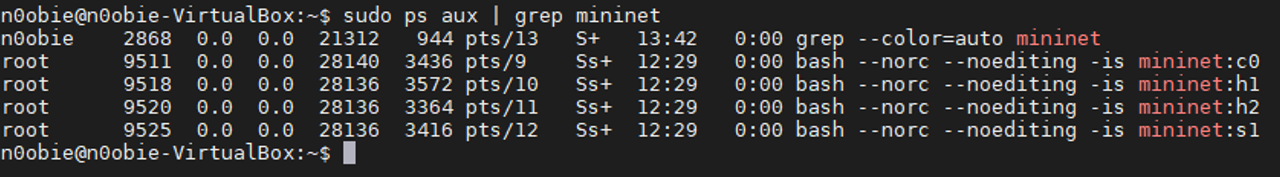
\includegraphics[width=\textwidth]{archivos/img/teoria/mn_03.png}
    \caption{Listado de procesos con referencias a Mininet}
    \label{fig:mininet_03}
\end{figure}

Si examinamos el archivo \texttt{/proc/{pid}/ns/net} para cada proceso mencionado en la figura \ref{fig:mininet_03}, podremos determinar cuáles de ellos se encuentran en una \textit{Network Namespace} distinta, según el valor del \textit{inode}. Por ejemplo, verifiquemos los procesos asociados a los \texttt{Host1} y \texttt{Host2}.\\


\begin{figure}[ht]
    \centering
    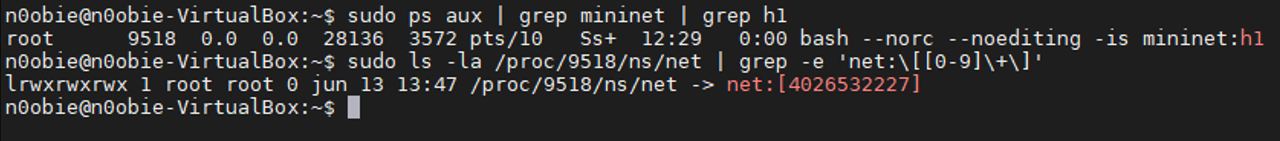
\includegraphics[width=\textwidth]{archivos/img/teoria/mn_04.png}
    \caption{Información de contexto sobre el proceso del Host1}
    \label{fig:mininet_04}
\end{figure}

\newpage

\begin{figure}[ht]
    \centering
    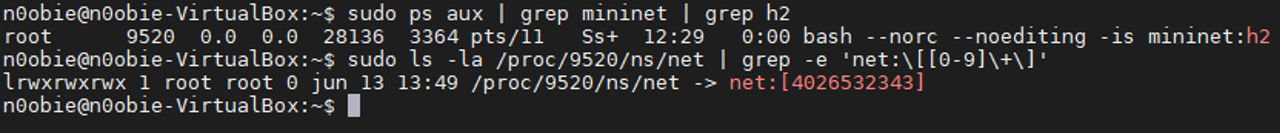
\includegraphics[width=\textwidth]{archivos/img/teoria/mn_05.png}
    \caption{Información de contexto sobre el proceso del Host2}
    \label{fig:mininet_05}
\end{figure}

Como se puede observar, hay diferentes \textit{inodes}, archivos distintos y \textit{Network namespaces} diferentes. Esta prueba demuestra cómo Mininet utiliza procesos de bash para mantener las \textit{Network Namespaces} de los nodos que lo requieren.


\subsection{Mininet-WiFi}

Mininet-WiFi \cite{7367387} es un emulador de redes inalámbricas diseñado principalmente para trabajar bajo el estándar \texttt{ieee80211}. Esta herramienta nació de Mininet, es decir, es un \textit{fork} de la misma. Por ello, comparten todas las bases sobre virtualización ``ligera" haciendo uso de \textit{Namespaces} y \gls{veth}s, por tanto, todos los scripts de Mininet son compatibles en Mininet-WiFi. \\
\par
Esto es así ya que toda la funcionalidad wireless es un añadido sobre la base que desarrollaron para Mininet. Los desarrolladores de Mininet-WiFi se valieron del subsistema wireless del Kernel de Linux y del módulo mac80211\_hwsim, para conseguir emular las interfaces y el supuesto medio inalámbrico. Para más información sobre esta herramienta se recomienda ir al \textbf{punto} \ref{mn-wifi_bmv2_integration}, donde se hace un análisis profundo sobre las jerarquías de clases añadidas en Mininet-WiFi, como opera internamente y como se comunica con el módulo en el kernel para generar los escenarios inalámbricos.



\subsection{Mininet-IoT}
\label{mininetIoT}

La herramienta Mininet-IoT \cite{mininetIOT} es un emulador de redes de baja capacidad diseñado para trabajar en conjunto bajo el estándar \texttt{ieee802154} y la capa de adaptación 6LoWPAN. Esta herramienta nació de Mininet-WiFi, que a su vez nació de Mininet, por lo que en la práctica, Mininet-IoT comparte todas las técnicas de virtualización ``ligera" de Mininet. Al heredar de Mininet-WiFi y Mininet, todos los scripts para desplegar topologías alámbricas y WiFi son compatibles en Mininet-IoT.  \\
\par

La gran diferencia entre Mininet-IoT y Mininet-WiFi, radica en el módulo que emplean para conseguir emular las interfaces y el supuesto medio inalámbrico. Mininet-WiFi hace uso del módulo mac80211\_hwsim, mientras que Mininet-IoT hace uso del módulo del Kernel mac802154\_hwsim (es necesario tener una versión del Kernel superior a la \texttt{4.18.x} para obtener dicho modulo). Toda la gestión de nodos, interfaces y enlaces es exactamente la misma a la de Mininet-WiFi. Por ello, Ramon Fontes (principal desarrollador de la herramienta), creó una clase agnóstica para gestionar módulos del Kernel en Mininet-WiFi, y migró todo el proyecto de Mininet-IoT a Mininet-WiFi. De esta forma, el mantenimiento del \textit{core} que compartían ambas herramientas se hacía únicamente en un proyecto, y daba la posibilidad al usuario de Mininet-WiFi de establecer enlaces de baja capacidad en sus topologías inalámbricas.